\documentclass[12pt]{article}                         
\pagestyle{plain}

\usepackage{amsmath}     % Enhanced math environments (e.g., align).
\usepackage{amsfonts}    % Math fonts (e.g., \mathfrak{}).
\usepackage{amstext}     % Text inside math mode (e.g., \text{where}).
\usepackage{amssymb}     % Extra math symbols (e.g., \mathbb{R}).
\usepackage{array}       % Advanced table/array column definitions.
\usepackage{circledtext} % Puts text inside a circle (e.g., \circledtext{A}).
\usepackage{comment}     % Include/exclude blocks of text.
\usepackage{enumerate}   % Customize itemized/numbered lists.
\usepackage{geometry}    % Adjusts page margins and layout.
\usepackage{graphicx}    % Include images/graphics (\includegraphics).
\usepackage{latexsym}    % Access to basic LaTeX symbols.
\usepackage{multicol}    % Allows text columns on a page.
\usepackage{pgfplots}    % Create scientific plots from data (based on TikZ).
\usepackage{tabularx}    % Tables that stretch to page width.
\usepackage{tasks}       % Create multi-column lists.
\usepackage{textcomp}    % Provides many text symbols (e.g., \textcelsius).
\usepackage{tikz}        % Create vector graphics and diagrams.
\usepackage{xcolor}      % Define and use colors.
\usepackage{fancyhdr}
\geometry{a4paper, margin=1in}
\pagestyle{fancy}
\fancyhf{} % Clear all header and footer fields
\fancyhead[L]{Your Name} % Left header with name
\fancyhead[R]{October 09th 2025} % Right header with date
\renewcommand{\headrulewidth}{0.4pt} % Horizontal line below the header

\begin{document}

% Main title
\begin{center}
    \Large \textbf{Math 115E Activity 11} \\
    \vspace{0.2cm}
    \normalsize Chapter 4 Section 2 \\
    \normalsize Determining slope from two points
\end{center}

\begin{center}   
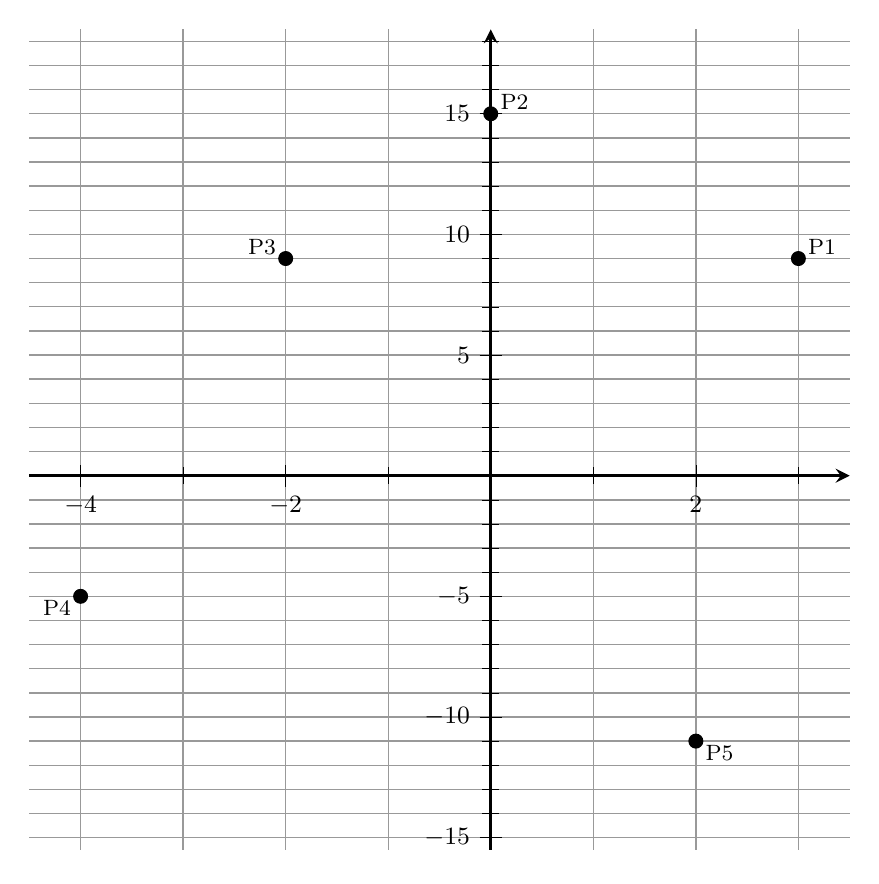
\begin{tikzpicture}
\begin{axis}[
    % Set the overall dimensions of the plot area
    height=12cm, 
    width=12cm,  
    % Set the domain and range for the axes
    xmin=-4.5, xmax=3.5,
    ymin=-15.5, ymax=18.5,
    % Manually set the tick marks
    xtick={-4,-2,0,2,4},
    ytick={-15,-10,-5,0,5,10,15,20},
    % Add 5 minor lines between each major tick on both axes
    minor x tick num=1,
    minor y tick num=4,
     % Axis and label styling
    axis lines=middle,
    tick label style={font=\small},
    % This command draws both major and minor grid lines
    grid=both,
    major grid style={line width=0.5pt,draw=gray!80},
    minor grid style={line width=0.5pt,draw=gray!80},
    % Axis and label styling
    axis lines=middle,
    tick style={draw=black, major tick length=8pt, minor tick length=6pt}, 
    xlabel style={at={(current axis.right of origin)}, anchor=west},
    ylabel style={at={(current axis.above origin)}, anchor=south},
    axis line style={-stealth, line width=1.2pt}
]

% --- LINES STARTING AT P1 (0, 15) ---
% 1. P1 to P2
%\draw[line width=1.5pt, draw=red]      (axis cs:0,15) -- (axis cs:3,9);
% 2. P1 to P3
%%\draw[line width=1.5pt, draw=blue]     (axis cs:0,15) -- (axis cs:-2,9);
% 3. P1 to P4
%\draw[line width=1.5pt, draw=green!70!black] (axis cs:0,15) -- (axis cs:-4,-5);
% 4. P1 to P5
%\draw[line width=1.5pt, draw=orange]   (axis cs:0,15) -- (axis cs:2,-11);

% --- LINES STARTING AT P2 (3, 9) ---
% 5. P2 to P3
%\draw[line width=1.5pt, draw=violet]   (axis cs:3,9) -- (axis cs:-2,9);
% 6. P2 to P4
%\draw[line width=1.5pt, draw=yellow!70!red] (axis cs:3,9) -- (axis cs:-4,-5); % Gold/Ochre
% 7. P2 to P5
%\draw[line width=1.5pt, draw=teal]     (axis cs:3,9) -- (axis cs:2,-11);

% --- LINES STARTING AT P3 (-2, 9) ---
% 8. P3 to P4
%\draw[line width=1.5pt, draw=magenta]  (axis cs:-2,9) -- (axis cs:-4,-5);
% 9. P3 to P5
%\draw[line width=1.5pt, draw=cyan]     (axis cs:-2,9) -- (axis cs:2,-11);

% --- LINE STARTING AT P4 (-4, -5) ---
% 10. P4 to P5
%\draw[line width=1.5pt, draw=lime]     (axis cs:-4,-5) -- (axis cs:2,-11);

% --- 2. PLOT ALL 5 POINTS (Markers) ---
\addplot[only marks, mark=*, black, mark size=2.5pt] 
    coordinates {
        (0,15)
        (3,9)
        (2,-11)
        (-4,-5)
        (-2,9)
    };

% --- 3. ADD LABELS (P1, P2, P3, P4, P5) ---
% Labels are positioned slightly above/below the points for clarity.
\node[right, font=\footnotesize] at (axis cs:3,9.5) {P1};
\node[right, font=\footnotesize] at (axis cs:0,15.5) {P2};
\node[left, font=\footnotesize] at (axis cs:-2,9.5) {P3};
\node[left, font=\footnotesize] at (axis cs:-4,-5.5) {P4};
\node[right, font=\footnotesize] at (axis cs:2,-11.5) {P5};

\end{axis}
\end{tikzpicture}
\end{center}

\newcolumntype{W}{>{\centering\arraybackslash}p{0.7cm}} 
\setcounter{section}{1}
\section{Value of the function beyond graph}
\begin{minipage}[t]{0.6\textwidth}
    \begin{enumerate}
        \item Find $f_1(4)$
        \\\\\\
        \item Find $f_2(10)$
        \\\\\\
        \item Find $f_3(1)$
        \\\\\\
        \item Find $f_4(-6)$
        \\\\\\
        \item Find $f_5(20)$
        
        
    \end{enumerate}
\end{minipage}
\begin{minipage}[t]{0.6\textwidth}
    \begin{enumerate}[\#1]
        \setcounter{enumi}{5} % continues numbering
        \item Find $f_6(0)$
        \\\\\\
        \item Find $f_7(-6)$
        \\\\\\
        \item Find $f_8(5)$
        \\\\\\
        \item Find $f_9(2)$
        \\\\\\
        \item Find $f_{10}(-12)$
        

    \end{enumerate}
\end{minipage}


\vspace{10cm}
\setcounter{section}{0}
\section{Find the equation of the line between two points}
\hspace{1cm} Find the equation of the line between the two points using Point-Slope Form
\par
\noindent
\hspace{1cm} then plot the function by connecting the corresponding dots above\\\\
\begin{minipage}[t]{0.6\textwidth}
    \begin{enumerate}
        \item $f_1(x)$=(P1-P2) =
        \\\\\\\\\\\\\\\\
        \item $f_2(x)$=(P1-P3) =
        \\\\\\\\\\\\\\\\
        \item $f_3(x)$=(P1-P4) =
        \\\\\\\\\\\\\\\\
        \item $f_4(x)$=(P1-P5) =
        \\\\\\\\\\\\\\\\
        \item $f_5(x)$=(P2-P3) =
        
        
    \end{enumerate}
\end{minipage}
\begin{minipage}[t]{0.6\textwidth}
    \begin{enumerate}[\#1]
        \setcounter{enumi}{5} % continues numbering
        \item $f_6(x)$=(P2-P4) =
        \\\\\\\\\\\\\\\\
        \item $f_7(x)$=(P2-P5) =
        \\\\\\\\\\\\\\\\
        \item $f_8(x)$=(P3-P4) =
        \\\\\\\\\\\\\\\\
        \item $f_9(x)$=(P3-P5) =
        \\\\\\\\\\\\\\\\
        \item $f_{10}(x)$=(P4-P5) =
        

    \end{enumerate}
\end{minipage}


\end{document}